\documentclass[a3paper 12pt]{article}

\usepackage[utf8]{inputenc}
\usepackage[T1]{fontenc}
\usepackage{mathptmx}
\usepackage{textcomp}
\usepackage[UKenglish]{babel}
\usepackage{amsmath, amssymb, mathtools}
\usepackage{float}
\usepackage[table]{xcolor}
\definecolor{backcolor}{rgb}{0.95,0.95,0.92}
\definecolor{codegreen}{rgb}{0,0.6,0}
\definecolor{codepurple}{rgb}{0.58,0,0.82}
\usepackage{listings}
\lstdefinestyle{code}{
	backgroundcolor=\color{backcolor},
	commentstyle=\color{codegreen},
	keywordstyle=\color{magenta},
	stringstyle=\color{codepurple},
	showspaces=false,
	showstringspaces=false,
	breaklines=true
}
\lstset{style=code}
\usepackage[hidelinks]{hyperref}
\hypersetup{
	colorlinks=false
}
\usepackage[style=ieee]{biblatex}
\bibliography{sources/biblio}
\renewcommand{\baselinestretch}{1.5}

\setlength{\parindent}{0pt}
\setlength{\parskip}{1em}

% figure support
\usepackage{import}
\usepackage{xifthen}
\pdfminorversion=7
\usepackage{pdfpages}
\usepackage{transparent}
\newcommand{\incfig}[1]{%
	\def\svgwidth{\columnwidth}
	\import{./figures/}{#1.pdf_tex}
}

\pdfsuppresswarningpagegroup=1

\begin{document}
\hypersetup{pageanchor=false}
\begin{titlepage}
  \begin{center}

    \textsc{\LARGE Dublin City University}\\[1cm]
    \textsc{\Large Electronic and Computer Engineering}\\[0.5cm]

    {\LARGE \bfseries Title\\[0.4cm]}
    {\Large \bfseries Subtitle\\[0.4cm]}

    \begin{figure}[H]
	
\includegraphics{images/Dcu-logo.png}
	\centering
    \end{figure}

    \vskip 2cm
    \emph{Author}\\[0.1cm]
    \noindent\makebox[\textwidth]{%
      \begin{tabular}{ll}%
        Michael Lenehan & michael.lenehan4@mail.dcu.ie \\
	Student Number: & 15410402 \\
    \end{tabular}}\\[0.1cm]

    \vfill

    % Bottom of the page
    % Probably replaced with date of deadline
    {\large{xx/xx/20xx}}

  \end{center}
\end{titlepage}

\hypersetup{pageanchor=true}
\pagenumbering{alph}
\thispagestyle{plain}
\begingroup
\renewcommand{\cleardoublepage}{}
\renewcommand{\clearpage}{}

\LARGE{Declaration}

\endgroup

\vskip 1cm

I declare that this material, which I now submit for assessment, is entirely my
own work and has not been taken from the work of others, save and to the extent
that such work has been cited and acknowledged within the text of my work. I
understand that plagiarism, collusion, and copying are grave and serious
offences in the university and accept the penalties that would be imposed should
I engage in plagiarism, collusion or copying. I have read and understood the
Assignment Regulations set out in the module documentation. I have identified
and included the source of all facts, ideas, opinions, and viewpoints of others
in the assignment references. Direct quotations from books, journal articles,
internet sources, module text, or any other source whatsoever are acknowledged
and the source cited are identified in the assignment references. This
assignment, or any part of it, has not been previously submitted by me or any
other person for assessment on this or any other course of study.

I have read and understood the DCU Academic Integrity and Plagiarism at
\url{https://www4.dcu.ie/sites/default/files/policy/1%20-%20integrity_and_plagiarism\_ovpaa_v3.pdf}
and IEEE referencing guidelines found at
\url{https://loop.dcu.ie/mod/url/view.php?id=448779}.

\vskip 1cm
Signed: \underline{\ \ \ \ \ \ \ \ \ \ \ \ \ \ \ \ \ \ \ \ \ \ \ \ \ \ \ \ \ \ \
\ \ \ \ \ \ } \hspace{20mm}Date: \underline{19/03/2020}

\hspace*{0mm}\phantom{Signed:}Michael Lenehan

\pagebreak

\pagenumbering{arabic}
\tableofcontents
\clearpage
\setlength{\abovedisplayskip}{-20pt}%
\setlength{\belowdisplayskip}{-10pt}%
\setlength{\abovedisplayshortskip}{0pt}%
\setlength{\belowdisplayshortskip}{0pt}%
\setlength{\jot}{0pt}% Inter-equation spacing
\section{Question 1}
In order to draw the feasible region, the following information is required:

\begin{align*}
	4x + y &\le 5 \\
	\therefore \text{Intersects axis at} (0,5) &\text{and} (1.25,0) \\
	5x - 2y &\le 3 \\
	\therefore \text{Intersects axis at} (0,-1.5) &\text{and} (0.6, 0) \\
	y &\le 3 \\
	\therefore \text{A line parallel to the x-axis at} y &= 3 \\
\end{align*}

It is also given that the feasible region occurs in the quadrant greater than
$x=-1$ and  $y=-1$.

\begin{figure}[H]
	\centering
	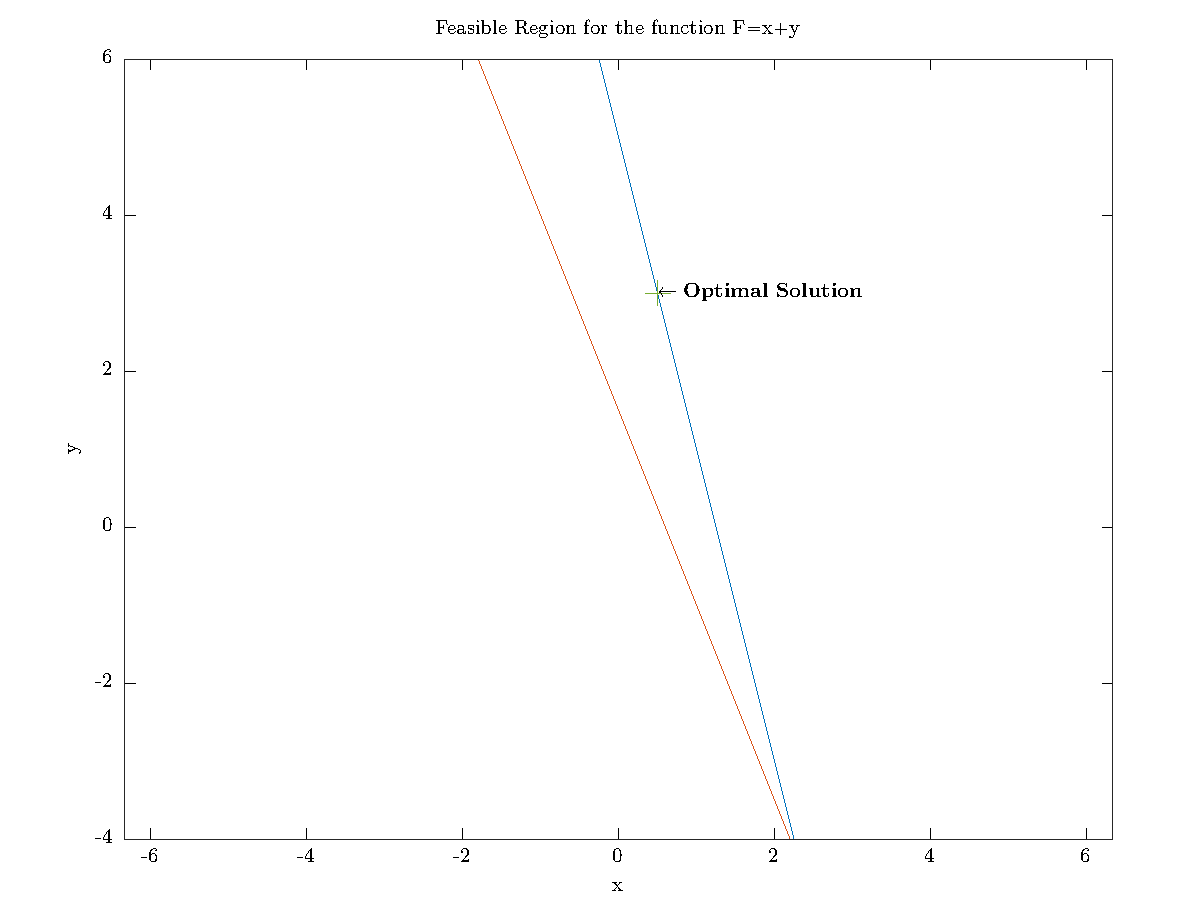
\includegraphics[width=\textwidth]{images/Q1}
	\caption{Feasible region for Q1}
	\label{fig:images-Q1}
\end{figure}

The maximum value is found to be at the point (0.5, 3.0).

If the objective function is changed to: minimise: $F=x$, the solution would be
(-1, 0), as the minimum value of x satisfies the objective function.

\section{Question 2}
\subsection{Part a}
It is not guaranteed that there will be a feasible solution to a Mixed
Dimensioning/Allocation Problem with Bounded Link Capacities. Because multiple
paths can have demands on the same links, the path flow variables are coupled.
If none of the link load values are equal to the link capacity values, a feasible
solution can be found. The shortest path allocation rule is used for
uncapacitated problems, i.e. problems where the demands do not ``compete'' for a
resource, in this case, the link. Therefore the Shortest Path Allocation Rule
does not apply to this problem.

\subsection{Part b}
The mixed problem is still a Linear Programming problem, as the objective
function, and the constraint equations are still linear functions of continuous
variables in $x$.

\subsection{Part c}
The demand volumes (in DVUs) are $h_1 = 14$ and $h_2 = 13$. The link capacities
are $c_1 = 12$,  $c_2 = 15$, and $c_3 = 3$.

In order to minimise the routing costs, try to route all traffic over direct
links. There is sufficient capacity to route demand volume  $h_2$ over direct
link, as the capacity is 15. This leaves an unused capacity of 2 on the link
$e=2$. Demand volume  $h_1$ can then be routed over link  $e=1$, with the
remaining demand volume routed over  $e=2$ and  $e=3$. This results in a
capacity of 1 remaining on link  $e=3$.

As such, the optimal values for ${x_d,p}$ are:

\begin{align*}
	x_{1,1} &= 12 \\
	x_{1,2} &= 2 \\
	x_{2,1} &= 13 \\
	x_{2,2} &= 0
\end{align*}

\subsection{Part d}
The link load ($y_e$) for each path-flow variable ($x_{d,p}$) is shown below:

\begin{align*}
	y_1 &= x_{1,1} + x_{2,2} \\
	    &= 12 + 0 \\
	    &= 12 \\
	y_2 &= x_{1,2} + x_{2,1} \\
	    &= 2 + 13 \\
	    &= 15 \\
	y_3 &= x_{1,2} \\
	    &= 2 \\
\end{align*}

\subsection{Part e}
Removing the capacity constraints, as with Question 4, would result in the same
outcome, with demand $h_3$ being bifurcated for an optimal solution. However,
there are solutions available in this situation which do not require this demand
to be split across links, such as by passing all of demand $h_3$ over path
$P_{3,2}$ or path $P_{1}$

\subsection{Part f}
Increasing the value of $\hat{h}_{1,2}$ to 15 would result in an infeasible
problem. While the capacity is available on link 3 for this increase in demand,
there is no availability for the increase on link 2. The available link capacity
remaining on $c_3$ is 1 DVU, which is the required amount for the increase in
demand, however there is 0 availability on the link $e=2$.

\section{Question 3}
\subsection{Part a}
It is not guaranteed that there will be a feasible solution to a Mixed
Dimensioning/Allocation Problem with Bounded Link Capacities. Because multiple
paths can have demands on the same links, the path flow variables are coupled.
If none of the link load values are equal to the link capacity values, a feasible
solution can be found. The shortest path allocation rule is used for
uncapacitated problems, i.e. problems where the demands do not ``compete'' for a
resource, in this case, the link. Therefore the Shortest Path Allocation Rule
does not apply to this problem.

\subsection{Part b}
The mixed problem is still a Linear Programming problem, as the objective
function, and the constraint equations are still linear functions of continuous
variables in $x$.

\section{Question 4}
\subsection{Part a}
It is not guaranteed that there will be a feasible solution to a Mixed
Dimensioning/Allocation Problem with Bounded Link Capacities. Because multiple
paths can have demands on the same links, the path flow variables are coupled.
If none of the link load values are equal to the link capacity values, a feasible
solution can be found. The shortest path allocation rule is used for
uncapacitated problems, i.e. problems where the demands do not ``compete'' for a
resource, in this case, the link. Therefore the Shortest Path Allocation Rule
does not apply to this problem.

\subsection{Part b}
The mixed problem is still a Linear Programming problem, as the objective
function, and the constraint equations are still linear functions of continuous
variables in $x$.

\section{Question 5}
\subsection{Part a}
It is not guaranteed that there will be a feasible solution to a Mixed
Dimensioning/Allocation Problem with Bounded Link Capacities. Because multiple
paths can have demands on the same links, the path flow variables are coupled.
If none of the link load values are equal to the link capacity values, a feasible
solution can be found. The shortest path allocation rule is used for
uncapacitated problems, i.e. problems where the demands do not ``compete'' for a
resource, in this case, the link. Therefore the Shortest Path Allocation Rule
does not apply to this problem.

\subsection{Part b}
The mixed problem is still a Linear Programming problem, as the objective
function, and the constraint equations are still linear functions of continuous
variables in $x$.

\subsection{Part c}
The demand volumes (in DVUs) are $h_1 = 14$ and $h_2 = 13$. The link capacities
are $c_1 = 12$,  $c_2 = 15$, and $c_3 = 3$.

In order to minimise the routing costs, try to route all traffic over direct
links. There is sufficient capacity to route demand volume  $h_2$ over direct
link, as the capacity is 15. This leaves an unused capacity of 2 on the link
$e=2$. Demand volume  $h_1$ can then be routed over link  $e=1$, with the
remaining demand volume routed over  $e=2$ and  $e=3$. This results in a
capacity of 1 remaining on link  $e=3$.

As such, the optimal values for ${x_d,p}$ are:

\begin{align*}
	x_{1,1} &= 12 \\
	x_{1,2} &= 2 \\
	x_{2,1} &= 13 \\
	x_{2,2} &= 0
\end{align*}

\section{Question 6}
\subsection{Part a}
It is not guaranteed that there will be a feasible solution to a Mixed
Dimensioning/Allocation Problem with Bounded Link Capacities. Because multiple
paths can have demands on the same links, the path flow variables are coupled.
If none of the link load values are equal to the link capacity values, a feasible
solution can be found. The shortest path allocation rule is used for
uncapacitated problems, i.e. problems where the demands do not ``compete'' for a
resource, in this case, the link. Therefore the Shortest Path Allocation Rule
does not apply to this problem.

\subsection{Part b}
The mixed problem is still a Linear Programming problem, as the objective
function, and the constraint equations are still linear functions of continuous
variables in $x$.

\subsection{Part c}
The demand volumes (in DVUs) are $h_1 = 14$ and $h_2 = 13$. The link capacities
are $c_1 = 12$,  $c_2 = 15$, and $c_3 = 3$.

In order to minimise the routing costs, try to route all traffic over direct
links. There is sufficient capacity to route demand volume  $h_2$ over direct
link, as the capacity is 15. This leaves an unused capacity of 2 on the link
$e=2$. Demand volume  $h_1$ can then be routed over link  $e=1$, with the
remaining demand volume routed over  $e=2$ and  $e=3$. This results in a
capacity of 1 remaining on link  $e=3$.

As such, the optimal values for ${x_d,p}$ are:

\begin{align*}
	x_{1,1} &= 12 \\
	x_{1,2} &= 2 \\
	x_{2,1} &= 13 \\
	x_{2,2} &= 0
\end{align*}

\subsection{Part d}
The link load ($y_e$) for each path-flow variable ($x_{d,p}$) is shown below:

\begin{align*}
	y_1 &= x_{1,1} + x_{2,2} \\
	    &= 12 + 0 \\
	    &= 12 \\
	y_2 &= x_{1,2} + x_{2,1} \\
	    &= 2 + 13 \\
	    &= 15 \\
	y_3 &= x_{1,2} \\
	    &= 2 \\
\end{align*}

\subsection{Part e}
Removing the capacity constraints, as with Question 4, would result in the same
outcome, with demand $h_3$ being bifurcated for an optimal solution. However,
there are solutions available in this situation which do not require this demand
to be split across links, such as by passing all of demand $h_3$ over path
$P_{3,2}$ or path $P_{1}$

\section{Question 7}
\lstinputlisting{Code/q7.lp}

The minimum value for the objective function obtained via this code is 127. The
demand is divided as follows:

\begin{align*}
	x_{1,1} &= 11 \\
	x_{1,2} &= 6 \\
	x_{2,1} &= 9 \\
	x_{2,2} &= 8 \\
	x_{3,1} &= 6 \\
	x_{3,2} &= 6
.\end{align*}

As can be seen from these path flow variables, there are no non-zero flows with
less than 6 demand volume units.

\section{Question 8}
\subsection{Part a}
It is not guaranteed that there will be a feasible solution to a Mixed
Dimensioning/Allocation Problem with Bounded Link Capacities. Because multiple
paths can have demands on the same links, the path flow variables are coupled.
If none of the link load values are equal to the link capacity values, a feasible
solution can be found. The shortest path allocation rule is used for
uncapacitated problems, i.e. problems where the demands do not ``compete'' for a
resource, in this case, the link. Therefore the Shortest Path Allocation Rule
does not apply to this problem.

\subsection{Part b}
The mixed problem is still a Linear Programming problem, as the objective
function, and the constraint equations are still linear functions of continuous
variables in $x$.

\section{Question 9}
\subsection{Part a}
It is not guaranteed that there will be a feasible solution to a Mixed
Dimensioning/Allocation Problem with Bounded Link Capacities. Because multiple
paths can have demands on the same links, the path flow variables are coupled.
If none of the link load values are equal to the link capacity values, a feasible
solution can be found. The shortest path allocation rule is used for
uncapacitated problems, i.e. problems where the demands do not ``compete'' for a
resource, in this case, the link. Therefore the Shortest Path Allocation Rule
does not apply to this problem.

\subsection{Part b}
The mixed problem is still a Linear Programming problem, as the objective
function, and the constraint equations are still linear functions of continuous
variables in $x$.

\section{Question 10}
\subsection{Part a}
It is not guaranteed that there will be a feasible solution to a Mixed
Dimensioning/Allocation Problem with Bounded Link Capacities. Because multiple
paths can have demands on the same links, the path flow variables are coupled.
If none of the link load values are equal to the link capacity values, a feasible
solution can be found. The shortest path allocation rule is used for
uncapacitated problems, i.e. problems where the demands do not ``compete'' for a
resource, in this case, the link. Therefore the Shortest Path Allocation Rule
does not apply to this problem.

\subsection{Part b}
The mixed problem is still a Linear Programming problem, as the objective
function, and the constraint equations are still linear functions of continuous
variables in $x$.

\clearpage
\printbibliography
\end{document}
